\section{Auswertung}
\label{sec:Auswertung}
\subsection{Vermessung von Spektrallinien}
\label{subsec:a0}
Es besteht die Möglichkeit allein durch Abzählen der Kanäle und der entsprechenden Zählergebnisse die Höhe, die Lage und den Inhalt einer Spektrallinie anzugeben.
Die Ergebnisse dieser Methode können jedoch nicht immer eindeutig angegeben werden, sodass eine unabhängige Auswertung unmöglich wird.
Hier wird daher eine andere Methode gewählt.
Zunächst wird die Lage einer Spektrallinie, wie oben auch, auf den Kanal mit dem höchsten Zählergebnis in einer hinreichend großen Umgebung geschätzt.
Um den so abgelesenen Kanal herum wird über die jeweils 20 oberhalb und unterhalb liegenden Kanäle eine Gauß-Funktion
\begin{align}
g(k)=c_1\exp\left(-c_2(k-c_3)^2\right)+c_4
\end{align}
an die Messdaten gefittet.
Dabei entspricht $c_1$ der Höhe der Spektrallinie und $c_3$ ihrer Lage.
Hier ist sofort ein Vorteil dieser Methode zu erkennen, denn die Lage einer Spektrallinie kann nun präziser als die Auflösung der Kanalskala angegeben werden.
Die Formel
\begin{align}
\int_\infty^\infty c_1\exp\left(-c_2(k-c_3)^2\right) dk = c_1 \sqrt{\frac{\pi}{c_2}}
\end{align}
zeigt, dass $c_1$ und $c_2$ zusammen ein Maß für den Inhalt einer Spektrallinie sind.
Der Parameter $c_4$ dient dazu Störeffekte wie das Compton-Kontinuum oder die Untergrundstrahlung aus den folgenden Rechnungen zu eliminieren.
Er wird deshalb im Folgenden nicht weiter berücksichtigt.
Diese und jede weitere Regressionsrechnung in dieser Auswertung wird mithilfe der Funktion \textit{curve\_ fit} aus dem Python Paket \textit{scipy.optimize} durchgeführt.
Fehlerrechnungen werden ebenfalls von Python übernommen. 
Dazu wird das Paket \textit{uncertainties} verwendet.

\subsection{Kallibration und Bestimmung der Effizienz}
\label{subsec:a1}
Um das Energiespektrum für unbekannte Strahler sinnvoll interpretieren zu können,
ist eine Kalibrierung der Energieskala notwendig. Dazu wird das linienreiche Spektrum eines Europium 152 Strahlers betrachtet, welches in Abbildung \ref{fig:spektrum_eu} dargestellt ist.
\begin{figure}
 \centering
 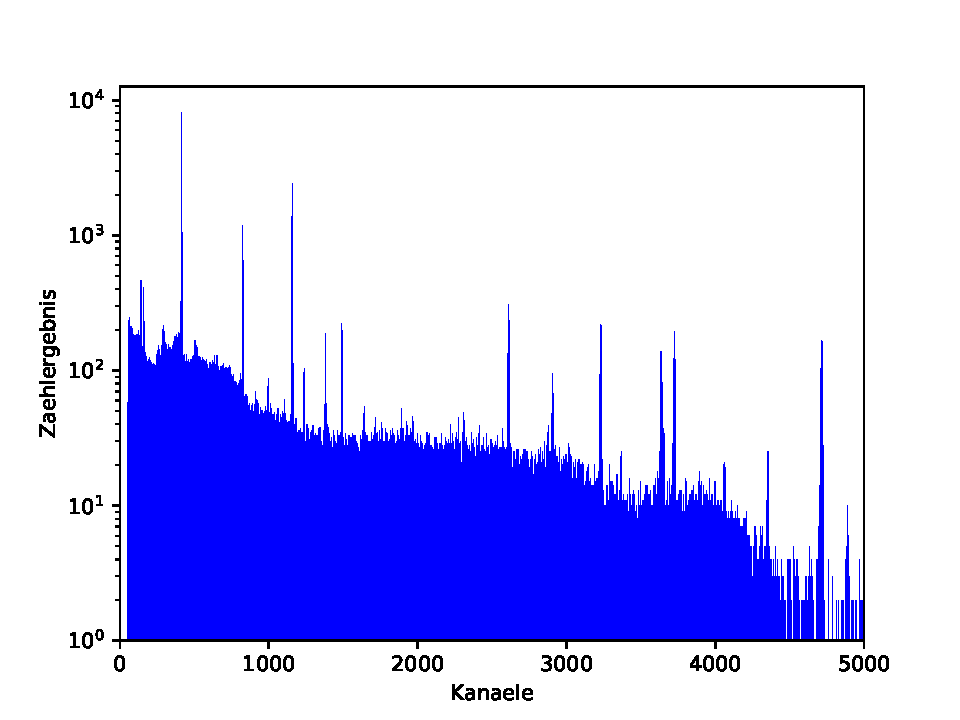
\includegraphics[width=0.8\textwidth]{python/plots/spec1.pdf}
 \caption{Rohdaten der Vermessung des Europium 152 Spektrums.}
 \label{fig:spektrum_eu}
 \end{figure} 
Die in Tabelle \ref{tab:atab1} angegebenen Lagen der Spektrallinien werden nach dem in Abschnitt \ref{subsec:a0} beschriebenen Verfahren bestimmt.
\begin{table}
\centering
\caption{Literaturwerte und gemessene Kanäle eines Europium 152 Gammaspektrums \cite{sample}.}
\begin{tabular}{c c c}
\hline \\
Kanal $k$ &Energie $E_\gamma$ in eV & Emissionswahrscheinlichkeit $W$ in \% \\
\hline \\
414.12 & 121.78 & 28.60 \\ 825.86 & 244.70 & 7.60 \\ 997.32 & 295.94 & 0.40 \\ 1158.71 & 344.30 & 26.50 \\ 1382.31 & 411.12 & 2.20 \\ 1491.59 & 443.96 & 3.10 \\ 2273.21 & 678.00 & 2.00 \\ 2310.43 & 688.67 & 0.90 \\ 2612.36 & 778.90 & 12.90 \\ 2908.55 & 867.37 & 4.20 \\ 3231.22 & 964.08 & 14.60 \\ 3368.59 & 1005.30 & 0.60 \\ 3639.40 & 1085.90 & 10.20 \\ 3726.07 & 1112.10 & 13.60 \\ 4353.21 & 1299.10 & 1.60 \\ 4716.58 & 1408.00 & 21.00 \\ 4888.94 & 1457.60 & 0.50 \\ 
\hline
\end{tabular}
\label{tab:atab1}
\end{table}
In Abbildung \ref{fig:Kalibrierung} werden die entsprechenden Kanäle gegen die Literaturwerte des Eu-Spektrums aufgetragen. 
Über eine lineare Ausgleichsrechnung wird die Umrechnungsvorschrift
\begin{align*}
k(E) = s \cdot E + b \text{, mit}\\
  s &= \SI{3.346+-0.001}{\per\electronvolt}\\
  b &= \SI{ 5.9+-0.8}{}
\end{align*}
zwischen Kanalnummern und Energien in eV bestimmt.
\begin{figure}
\centering
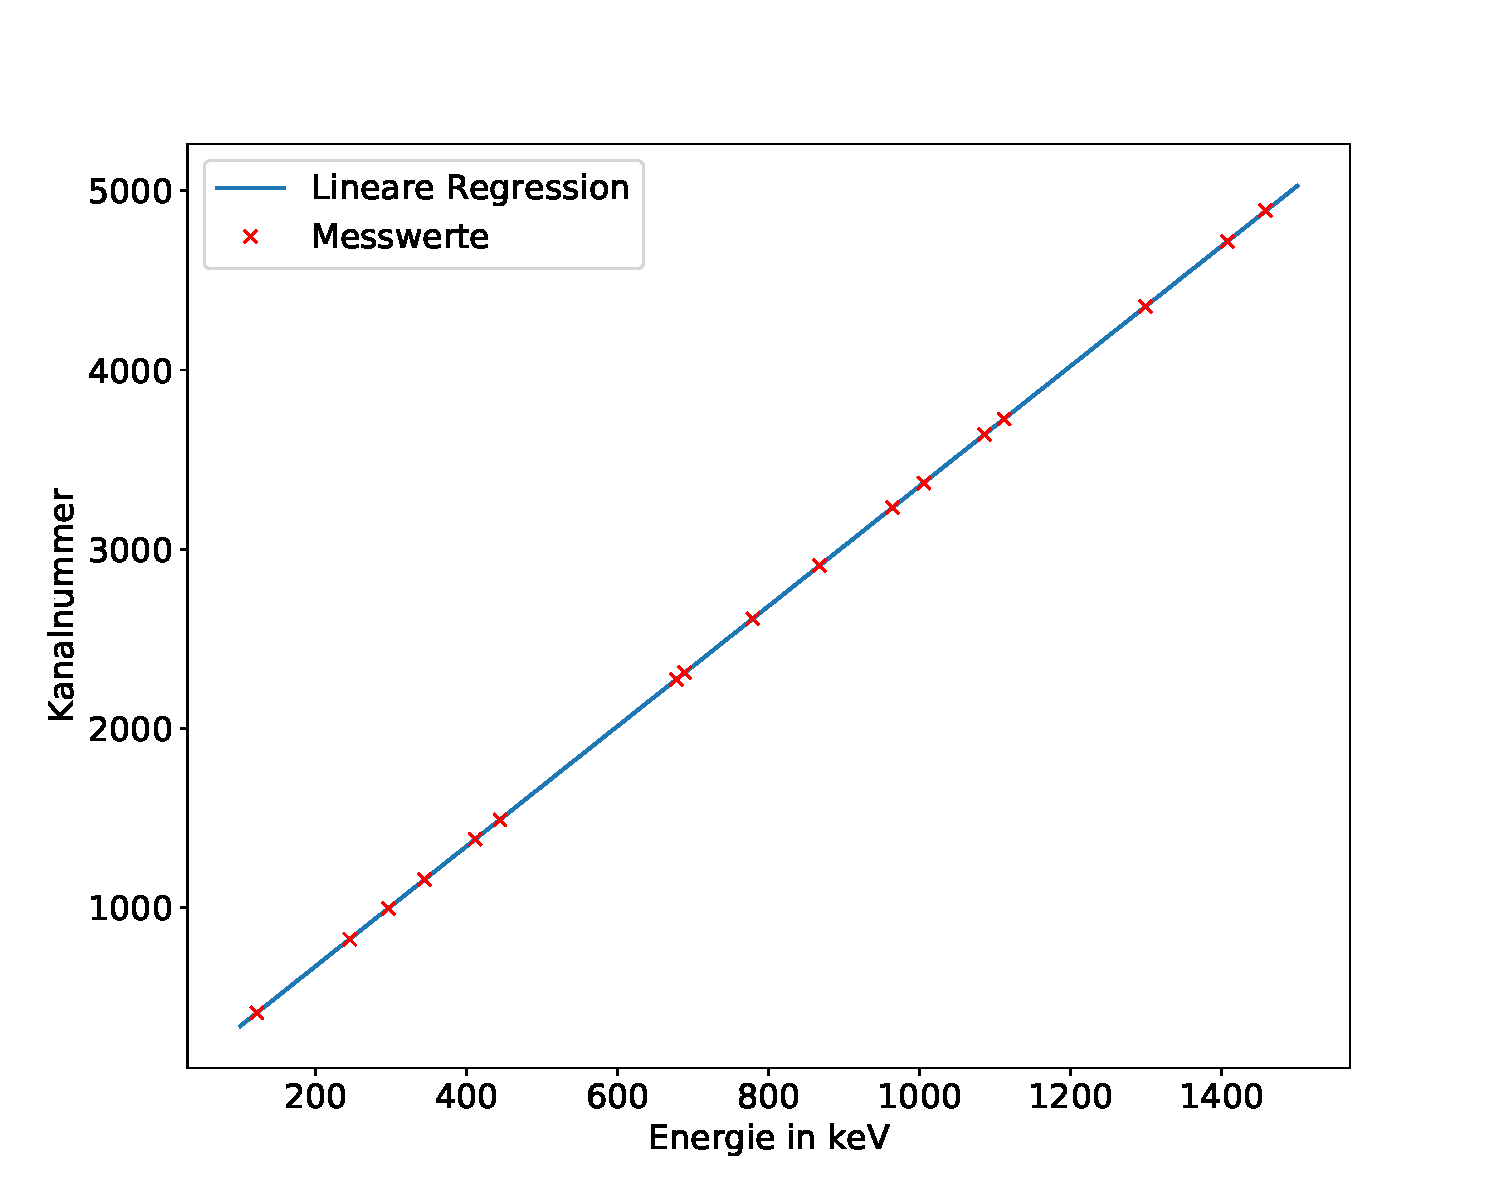
\includegraphics[width=0.8\textwidth]{python/plots/kalibrierung.pdf}
\caption{Lineare Regression der Messwerte aus Tabelle \ref{tab:atab1}}
\label{fig:Kalibrierung}
\end{figure}
Mit Gleichung \eqref{eqn:anleitung22} soll die Effizienz der Spektrallinien berechnet werden.
Um die dazu nötige Aktivität des Europiums zum Zeitpunkt der Messung zu bestimmen, wird das exponentielle Zerfallsgesetz
\begin{align}
A_\text{Messung}=A_0\exp\left(\frac{\log(2)}{T_{\frac{1}{2}}}\Delta t\right)
\end{align}
verwendet.
Die Aktivität $A_0$ am 01.10.2000 betrug $\SI{130+-60}{\becquerel}$ und die Halbwertszeit von Europium beträgt $\SI{4943+-5}{\day}$ \cite{sample}.
Das angegebene Datum liefert eine zeitliche Differenz von $\Delta t=\SI{6084}{\day}$, sodass sich eine Aktivität von 
\begin{align*}
A_\text{Messung}=\SI{1760+-26}{\becquerel}
\end{align*}
ergibt.
Leider wurde der Abstand $d$ zwischen Probe und Detektor nicht gemessen. 
Der Wert von $d=\SI{8.8+-0.3}{\centi\meter}$ wird deshalb dem Protokoll einer befreundeten Gruppe entnommen \cite{abstand}.
Der Radius der Probe beträgt $r=\SI{2.25}{\centi\meter}$ \cite{sample}.
Aus
\begin{align}
\frac{\Omega}{4\pi}=\frac{1}{2}\left( 1- \frac{d}{\sqrt{d^2+r^2}}\right)
\end{align}
lässt sich dann der Raumwinkel $\Omega=\SI{1.96+-0.021}{}$ berechnen.
Mit diesem Wert und den aus den Gauß-Fits berechneten Flächeninhalten der Gauß-Funktionen lassen sich nun die in Tabelle \ref{tab:atab2} angegebenen Effizienzen berechnen.
Dabei ist zu Berücksichtigen, dass die Zählrate aus Formel \ref{eqn:anleitung22} gerade den Inhalten geteilt durch die Messdauer $t_\text{Messung}=\SI{7764}{\second}$ entspricht.
\begin{table}
\centering
\caption{Inhalte der Gauß-Fits und die daraus berechneten Effizienzen.}
\begin{tabular}{c c c}
\hline \\
Energie in $\SI{}{\electronvolt}$ & Inhalt & Effizienz in \%\\
\hline \\
121.78 & 28310$\pm$90 & 45.5$\pm$0.6 \\ 244.70 & 4770$\pm$40 & 28.80$\pm$0.5 \\ 295.94 & 230$\pm$30 & 27.0$\pm$3.0 \\ 344.30 & 11700$\pm$70 & 20.3$\pm$0.3 \\ 411.12 & 740$\pm$20 & 15.4$\pm$0.5 \\ 443.96 & 1010$\pm$20 & 15.0$\pm$0.4 \\ 678.00 & 40$\pm$10 & 1.00$\pm$0.3 \\ 688.67 & 240$\pm$20 & 12.0$\pm$1.0 \\ 778.90 & 2320$\pm$40 & 8.3$\pm$0.2 \\ 867.37 & 640$\pm$30 & 7.0$\pm$0.3 \\ 964.08 & 2080$\pm$40 & 6.6$\pm$0.2 \\ 1005.30 & 90$\pm$10 & 7.0$\pm$1.0 \\ 1085.90 & 1170$\pm$40 & 5.3$\pm$0.2 \\ 1112.10 & 1830$\pm$40 & 6.2$\pm$0.2 \\ 1299.10 & 160$\pm$20 & 4.6$\pm$0.5 \\ 1408.00 & 2290$\pm$70 & 5.0$\pm$0.2 \\ 1457.60 & 180$\pm$50 & 16.0$\pm$5.0\\
\hline
\end{tabular}
\label{tab:atab2}
\end{table}
Es wird angenommen, dass die Effizienz $Q$ mit steigender Energie wie eine Potenzfunktion
\begin{align}
Q(E)=c E^{d}
\end{align}
abnimmt.
Die in Abbildung \ref{fig:Effizienz} dargestellte Regressionsrechnung liefert die Parameter
\begin{align*}
c&=\SI{80+-40}{}\\
d&=\SI{-1.03+-0.07}{}\text{ .}
\end{align*}
\begin{figure}
\centering
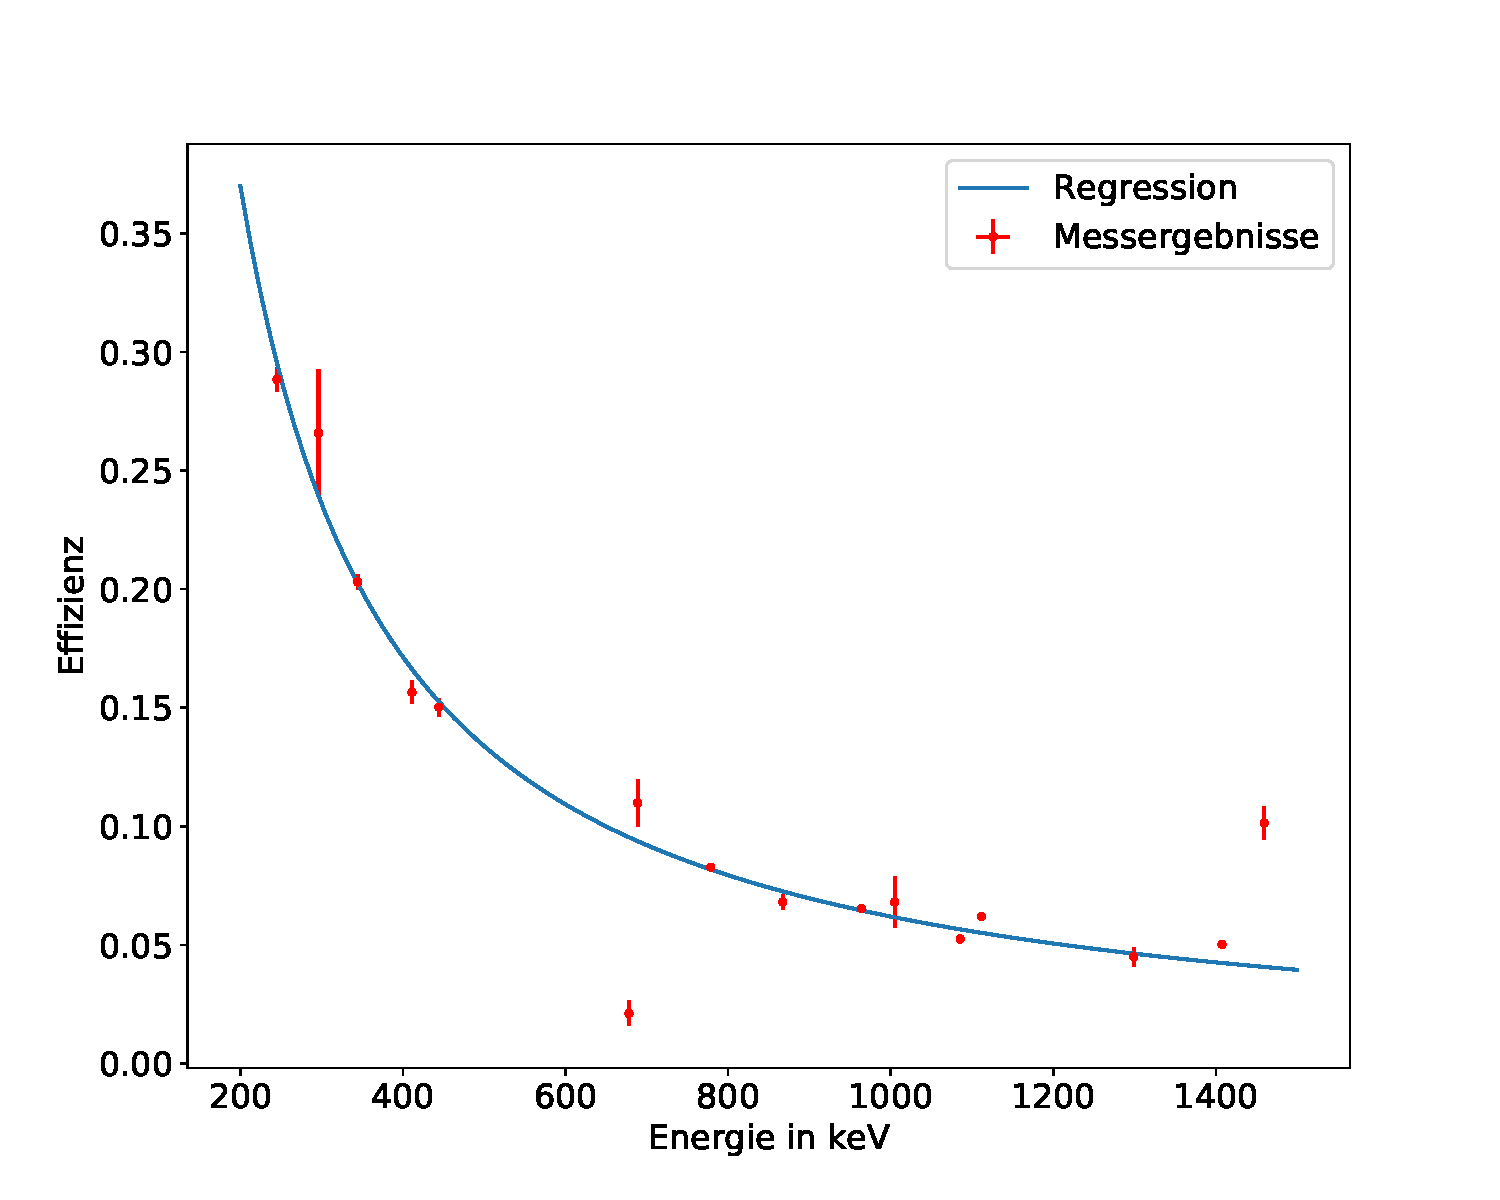
\includegraphics[width=0.8\textwidth]{python/plots/effizienz.pdf}
\caption{Darstellung der Abnahme der Effizienz mit Steigender Energie durch eine Regressionsrechnung. Energien unterhalb von $\SI{150}{\electronvolt}$ werden nicht betrachtet.}
Dabei wird der Peak bei ca. $\SI{778}{\electronvolt}$ vernachlässigt, da eine Inhaltsbestimmung wegen des Untergrunds kaum möglich ist.
\label{fig:Effizienz}
\end{figure}
\subsection{Bestimmungen von Detektoreigenschaften}
\label{subsec:a2}






\subsection{Aktivitätsbestimmung von Barium 133}
\label{subsec:a3}
In Abbildung \ref{fig:Spektrum_Barium} ist das Spektrum einer Barium 133 Probe dargestellt.
\begin{figure}
\centering
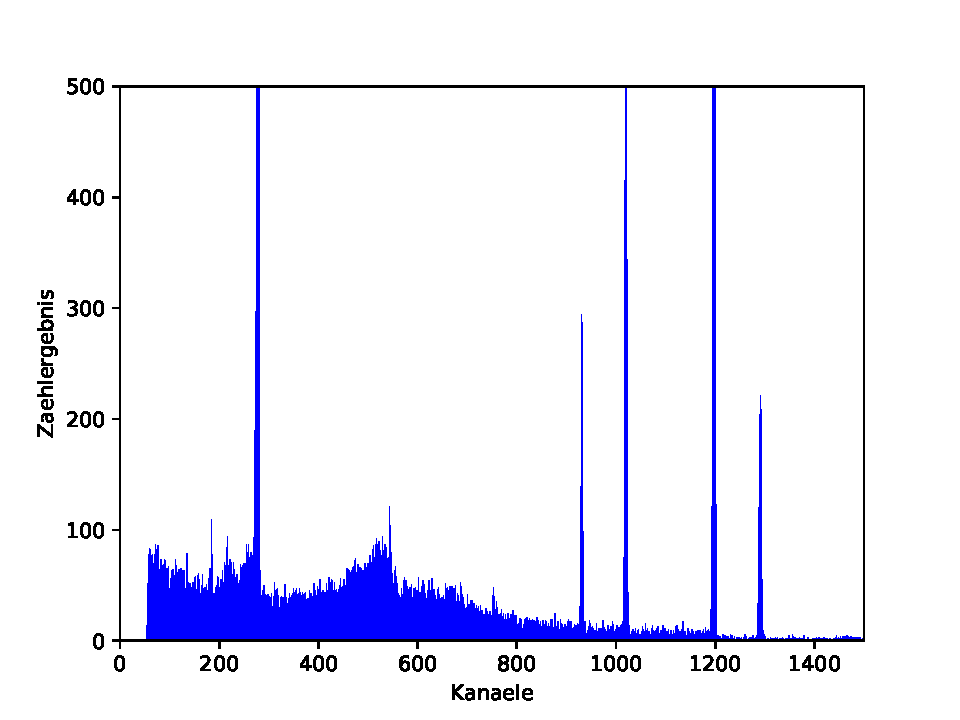
\includegraphics[width=0.8\textwidth]{python/plots/spec3.pdf}
\caption{Gamma-Spektrum einer Barium 133 Probe.}
\label{fig:Spektrum_Barium}
\end{figure}
Um die Aktivität der Probe zum Zeitpunkt der Messung zu bestimmen wird Gleichung (\ref{eqn:anleitung22}) verwendet.
Wie in Abschnitt \ref{subsec:a0} beschrieben wird die Lage und der Inhalt der verschiedenen Peaks berechnet.
Mit der in Abschnitt \ref{subsec:a1} bestimmten Beziehung $Q(E)$ zwischen Effizienz und Energie, dem bekannten Raumwinkel $\Omega$ und den in Tabelle \ref{tab:a_d_1} angegebenen Emissionswahrscheinlichkeiten wird von jeder Spektrallinie einzeln auf die Aktivität der Probe geschlossen.
Die Ergebnisse dieser Rechnung finden sich ebenfalls in Tabelle \ref{tab:a_d_1}.
\begin{table}
\centering
\caption{Für die Berechnung der Aktivität wichtige Daten je Spektrallinie.}
\begin{tabular}{c c c c}
\hline \\
Lage in eV & Intensität in s$^{-1}$&  Emissionswahrscheinlichkeit in \%& Aktivität in $\SI{}{\becquerel}$\\
\hline \\
184.93 $\pm$0.15  &  0.04  $\pm$0.02  &  2.20  &  102  $\pm$57 \\ 278.34 $\pm$0.02  &  2.93  $\pm$1.59  &  34.06  &  540  $\pm$293 \\ 543.81 $\pm$0.32  &  0.14  $\pm$0.10  &  0.65  &  1365  $\pm$919 \\ 753.17 $\pm$0.15  &  0.08  $\pm$0.05  &  0.45  &  1101  $\pm$678 \\ 931.69 $\pm$0.02  &  1.54  $\pm$0.92  &  7.20  &  1341  $\pm$804 \\ 1020.80 $\pm$0.03  &  3.96  $\pm$2.40  &  18.30  &  1360  $\pm$822 \\ 1198.10 $\pm$0.01  &  13.29  $\pm$8.14  &  62.10  &  1344  $\pm$823 \\ 1291.30 $\pm$0.05  &  1.96  $\pm$1.21  &  8.90  &  1382  $\pm$853 \\ 
\hline
\end{tabular}
\label{tab:a_d_1}
\end{table}
Als Mittelwert dieser einzelnen Aktivitäten ergibt sich das gesamt Ergebnis der Aktivität 
\begin{align*}
A_{Ba-133}=\SI{1320+-100}{\becquerel} \text{ .}
\end{align*}
Die Aktivitäten, welche aus den ersten beiden Spektrallinien berechnet werden, werden bei dieser Rechnung vernachlässigt.
\subsection{Untersuchung von Zerfallsketten in }
\label{subsec:a4}



%\begin{figure}
%  \centering
%  \includegraphics{plot.pdf}
%  \caption{Plot.}
%  \label{fig:plot}
%\end{figure}
